\section{Supervised Learning}
A Neural networks are AI computational systems that are 'inspired' by biological neural systems. Their main feature is the abiblity to learn from the expericnece with using examples of classification.
\\\\
A single neuron is a linear classifier, classification can be thought as a way of separating the input data.


\subsection{Perceptron}
This is a machine learning algorithm that helps provide classified outcomes for computing. It dates back to the 1950s and represents a fundamental example of how machine learning algorithms work to develop data structure. This algorithms was invented by Frank Rosenblatt, it has an input and an output layer, a binary activation function. Update rule based on Hebbian learning: connections that are active at the same time are strengthen.
\\\\
The basic of the algorithm is four parts.
\begin{itemize}
    \item Setup: Weights are randomly assigned typically between -0.5 and 0.5
    \item Inputs: $x_1, x_2,..,x_n$; binary (0/1)
    \item Connection Strengths: $w_1,w_2,...,w_n$ and bias $\theta$
    \item Summation $ h = \sum_{i=1}^{n} w_i x_i$
    \item Output $y = f(h-\theta)$; binary: if $h > T$ then $y = 0$ else $y =1$
\end{itemize}
A Perceptron is a linear classification. Therefore the linear separator between two classes on a 2d plane is $x_2 = kx_1+b$ where $k = \frac{w_1}{w_2}$ as $x_2$ can be written as $x_2 = -\frac{w_1}{w_2}x_1 + \frac{\theta}{w_2}$
\subsubsection{Learning rule: training perceptron}
In a general case, to adjust weights $w$ and the bias $\theta$ of the perceptron, the learning (training) procedure is used. The training set includes many pairs, the input vector $x$ and the targeted output $t(x,t)$ We send one input vector $x$ to the perceptron adn the the actual output is $O$. The learning rule to adjust weights and bias is based on the difference (error) between the actual output $O$ and the targeted value $t:error = t-O$
\begin{itemize}
    \item Error: $e= t-O$
    \item $W_{new} = W_{old} +qx(t-O)$
    \item $\theta_{new} \theta_{old} + q(t-O)$
    \item Where $0<q<1$is the learning rate
\end{itemize}
This is also know as the Hebbian learning algorithms and mathematical equation is as follows.
\begin{equation}
    W_{ij}[n+1] = W_{ij}[n] + \eta x_i[n]x_j[n]
\end{equation}
Where $\eta$ is the learning rate coefficient and $x$ are the outputs of the $i$th and $j$th elements.
\subsubsection{Example}
Lets examine a simple example to help see how a perceptron can learn to represent the logical-OR function for two inputs, using a threshold of zero $t = 0$ and a learning rate $\eta$ of 0.2.
\begin{itemize}
    \item First we need set the associated weights which for this example will be $w_1 = -0.2$ and $w_2=0.4$
    \item Now, the first epoch is run through, the training data will consist of the four combinations of 1's and 0's possible with two inputs. Hence, our first piece of training data is $x_1 = 0$ and $x_2 = 0$ and our expected outcome is 0
    \item So we apply the formula $ h = \sum_{i=1}^{n} w_i x_i$
    \item resulting in $h = 0$
    \item since $h$ is as expected, and the error, $e$, is therefore 0, the weights do not change.
    \item Now $x_1 = 0$ and $x_2 =1$ and our expected outcome is 1
    \item Apply the formula and we get $h=0.4$
    \item So the output is 1, so the weights don't need to change
    \item Now $x_1 = 1$ and $x_2 =0$ and our expected outcome is 1
    \item Apply the formula and we get $h=-0.2$
    \item So the output is 0, so the weights need to change as the expected output was 1
    \item So we apply the perceptron training rule to assign new values to the weights, using the predefined $\eta$ and this case $e$ is 1.
    \item $w_1 = -0.2(0.2\cdot1\cdot1)$,  $w_1 = 0$
    \item $w_2 = 0.4(0.2\cdot0\cdot1)$,  $w_1 = 0.4$ as this did not contribute to this error it is not adjusted.
    \item Now $x_1 = 1$ and $x_2 =1$ and our expected outcome is 1
    \item Apply the formula and we get $h=0.4$
    \item So the output is 1, so the weights don't need to change
    \item This is the end of the first epoch, and at this point the method runs again and continues to repeat until all four piece of training data are classified correctly. 
\end{itemize}
\subsubsection{Limitations}
The exclusive OR function cannot be modeled using a perceptron. This is because the perceptrons can only learn to model functions that are linearly separable.
\subsection{Multilayer Perceptron}
An artificial neural network (ANN) consists of a set of interconnected nodes. ANN is able to receive inputs from the environment and to learn new behaviours (responses)
\subsubsection{ANN: forward pass} 
A ANN: forward pass is similar to a perceptron, the unit output is given by the weighted sum of the inputs, passed through an activation function. 
\begin{figure}[htbp]
    \centering
    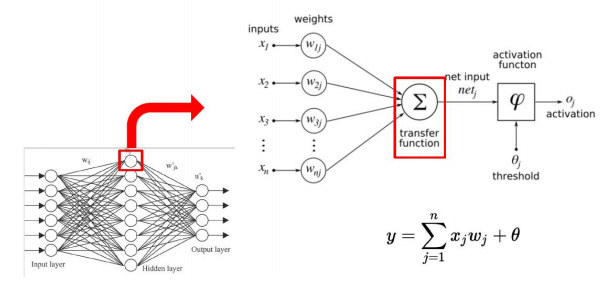
\includegraphics[width= \textwidth]{Images/ANNFowardPass.PNG}
    \caption{Hidden node}
    \label{fig`:dendrogram}
\end{figure}
\smallskip
\subsubsection{ANN: backward pass (error estimation)}
The performance of the network is evaluated using a loss function which must be differentiable. Generally an L2 norm is used the output is then compared with the expected value. The expected value is given by the label associated with the input and is stored in the data set. 
\begin{figure}[!htbp]
    \centering
    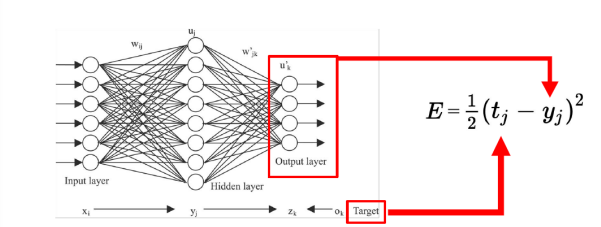
\includegraphics[width= \textwidth]{Images/OutputLayer.PNG}
    \caption{Output node}
    \label{fig`:dendrogram}
\end{figure}
\smallskip
\subsubsection{ANN: backward pass (update rule)}
The standard approach for training an ANN is back-propagation this is based on gradient descent, at each iteration the weights are adjusted in order to obtain an output that is more similar to the target. It is important to select the right hyper-parameters (e.g. learning rate).
\begin{figure}[!htbp]
    \centering
    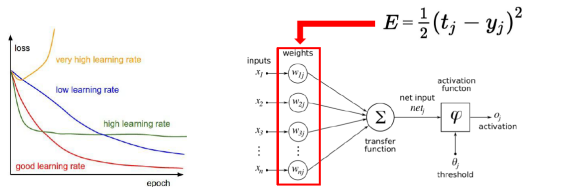
\includegraphics[width= \textwidth]{Images/UpdateRule.PNG}
    \caption{Update weights}
    \label{fig`:dendrogram}
\end{figure}
\smallskip
\subsubsection{Activation functions}
An activation function of a node defines the output of that node. It maps the resulting values into the desired range such as between 0 to 1 or -1 to 1 etc. (depending upon the choice of activation function). For example, the use of the logistic activation function would map all inputs in the real number domain into the range of 0 to 1, depending upon the choice of activation function.
\subsubsubsection{Sigmoid activation function}
This is a mathematical function that has the characteristic of an "S"-shaped curve. Often the sigmoid function refers to a special case of the logistic function. \\\\
The definition of a sigmoid functions is as follows. 
\begin{center}
    \textbf{A sigmoid function is bounded, differential, real function that is defined for all real input values and has a non-negative derivative at each point.}
\end{center}
In general, a sigmoid function is monotonic, and has a first derivative which is bell shaped. A sigmoid function is constrained by a pair of horizontal asymptotes as {\displaystyle x\rightarrow \pm \infty }
\subsubsection{ANN with hidden layers}
 The training data (input array and target output) should be
used to adjust parameters of ANN classifier,the learning procedure is based on minimization of the
total (for all training data) error function which depends on
training data and many parameters (weights and biases. Minimization is based on the idea of the gradient descend method. To minimize computational time, the idea of
backpropagation is used: moving backward (from output to input though several hidden layers) pick up already calculated components of the gradient and use them to
adjust ANN parameters.
\subsection{Support Vector Machine Binary Classifier}
A support vector machine constructs a hyper-plane or set of hyper planes in high or infinite-dimensional space known as the decision boundary in (2 dimensional space this is a line), the distance between hyper-planes is know as the margin. The goal is to find the decision boundary with maximal margin! A good hyper-plane is equidistant from both classes. A support Vector are data points that the margin pushes up against. 
\subsubsubsection{SVM as Nonlinear classifier's }
SMV can be applied to data of complex non linear structure, for this type of classification data transformation (kernel) is used, the SMV can be used to classify data to several classes, for that a set of binary SVM is combined to produce the best solution for a multi class problem.